\documentclass[aspectratio=169]{beamer}

\mode<presentation>
\usetheme{Boadilla}
\definecolor{NTHU1}{RGB}{127,16,132}
\definecolor{NTHU2}{RGB}{228,210,231}
\definecolor{blue}{RGB}{30,90,205}
\definecolor{red}{RGB}{213,94,0}
\definecolor{green}{RGB}{0,128,0}
\definecolor{charcoalgray}{RGB}{108,104,104}
\setbeamercolor{title}{fg=NTHU1}
\setbeamercolor{frametitle}{fg=NTHU1}
\setbeamercolor{block title}{bg=NTHU1, fg=white}
\setbeamercolor{block body}{bg=NTHU2}
\setbeamercolor{structure}{fg=NTHU1}
\setbeamercolor{item projected}{fg=white}
\setbeamercolor{item}{fg=NTHU1}
\setbeamercolor{subitem}{fg=NTHU1}
\setbeamercolor{section in toc}{fg=NTHU1}
\setbeamercolor{description item}{fg=NTHU1}
\setbeamercolor{caption name}{fg=NTHU1}
\setbeamercolor{button}{bg=NTHU1, fg=white}
\setbeamercolor{caption name}{fg=NTHU1}
\usepackage{graphics}
\usepackage{tikz}
\usepackage{amsmath}
\usepackage{bbm}
\usetikzlibrary{decorations.pathreplacing}
\usepackage{geometry}
\usepackage{booktabs}
\usepackage{bookmark}
\usepackage{multirow, makecell}
\usepackage{float}
\usepackage{fancyvrb}
\usepackage{caption}
\captionsetup[figure]{singlelinecheck = false, format= hang, justification=centering}
\captionsetup[subfigure]{singlelinecheck = false, format= hang, justification=raggedright}
\usepackage{subcaption}
\usepackage{adjustbox}
\usepackage{hyperref}
\usepackage{threeparttable}
\usepackage{appendixnumberbeamer} 
\usepackage[T1]{fontenc}
\usepackage[default]{lato} 
\usepackage{smartdiagram}
\smartdiagramset{
  back arrow disabled = true,
  module minimum width=1cm,
  module x sep = 3,
  uniform arrow color=true,
}
\usepackage{xcolor}
\usepackage{colortbl}
	\definecolor{light-gray}{gray}{0.99}

\newenvironment{wideitemize}{\itemize\addtolength{\itemsep}{10pt}}{\enditemize}
\newenvironment{wideenumerate}{\enumerate\addtolength{\itemsep}{10pt}}{\endenumerate}
\newenvironment{widedescription}{\description\addtolength{\itemsep}{10pt}}{\enddescription}
\hypersetup{
colorlinks=true,
linkcolor=NTHU1,
filecolor=green, 
urlcolor=blue,
}
\beamertemplatenavigationsymbolsempty
\setbeamercolor{author in head/foot}{bg=white, fg=NTHU1}
\setbeamercolor{title in head/foot}{bg=white, fg=NTHU1}
\setbeamercolor{date in head/foot}{bg=white, fg=NTHU1}
\setbeamercolor{section in head/foot}{bg=white, fg=NTHU1}
\setbeamercolor{headline}{bg=white}
\setbeamertemplate{footline}{
    \leavevmode%
    \hbox{%
        \begin{beamercolorbox}[wd=.333333\paperwidth,ht=2.25ex,dp=1ex,center]{date in head/foot}%
            \usebeamerfont{date in head/foot}%\insertdate
        \end{beamercolorbox}%
        \begin{beamercolorbox}[wd=.333333\paperwidth,ht=2.25ex,dp=1ex,center]{title in head/foot}%
            \usebeamerfont{title in head/foot}\insertshorttitle
        \end{beamercolorbox}%
        \begin{beamercolorbox}[wd=.333333\paperwidth,ht=2.25ex,dp=1ex,right]{date in head/foot}%
            \usebeamerfont{date in head/foot}\insertframenumber{}\hspace*{2em}
        \end{beamercolorbox}}%
        \vskip0pt%
    }
    %% May need to script the introduction!!!!!!
%\setbeamercolor{page number in head/foot}{fg=NTHU1}
\setbeamertemplate{section in toc}[sections numbered]
\setbeamertemplate{subsection in toc}{\leavevmode\leftskip=3em\rlap{\hskip-1.75em\inserttocsectionnumber.\inserttocsubsectionnumber}
\inserttocsubsection\par}
\setbeamerfont{subsection in toc}{size=\footnotesize}
%\setbeamertemplate{headline}{%
  %\begin{beamercolorbox}[ht=5.5ex]{section in head/foot}
    %\vskip2pt\insertnavigation{0.33\paperwidth}\vskip2pt
  %\end{beamercolorbox}%
%}
\newenvironment{transitionframe}{\setbeamercolor{background canvas}{bg=white}\setbeamertemplate{footline}{} \begin{frame}[noframenumbering]}{\end{frame}}


\makeatletter
\let\@@magyar@captionfix\relax
\makeatother


\title[]{Public Economics and Development} % Change this regularly
\subtitle[]{Week 5: Theories on Provision of Public Goods}
\author[Lee]{Seung-hun Lee }
\institute[]{Taipei School of Economics\\ National Tsing Hua University}

\date[]{April 7th, 2026}

\begin{document}
\begin{transitionframe}
\titlepage
\end{transitionframe}


%%% Color slides for section headers: Use for colloquium version (The ones bewteen \iffals and \fi)
\begin{transitionframe}
\frametitle{Roadmap for today}
\tableofcontents
\end{transitionframe}


\section{Market failure and the role of the government}
\begin{frame}
\frametitle{Where does the money raised by government go to} 
Previous lecture: How to set tax system to optimally collect money
\begin{itemize}\setlength\itemsep{3pt}
\item Maximizing social welfare
\item With respect to meeting the revenue requirment or budget constraint
\item Often comes with efficiency loss \textit{when compared to perfectly competitive outcomes}
\end{itemize}\medskip
Why do government want to raise money? Correct for market failures
\begin{itemize}\setlength\itemsep{3pt}
\item Markets may not be competitive - monopolies and oligopolies
\item There are incomplete information - asymmetric information
\item Markets under/over produce some goods (e.g. public goods) - externalities
\item Markets may generate inequitable outcomes - redistribution
\end{itemize}
\medskip
We focus on public goods \& redistribution, and discuss management of public institutions
\end{frame}

\begin{frame}
\frametitle{Imperfect competition} 
\begin{columns}
\begin{column}{0.5\textwidth}
  \begin{center}
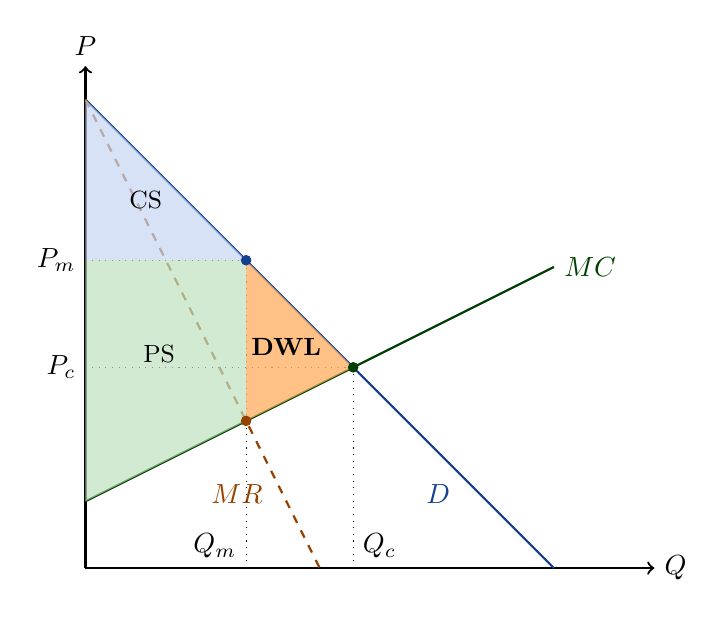
\begin{tikzpicture}[scale=0.85]

% Axes
\draw[->,thick] (0,0) -- (8.5,0) node[right] {$Q$};
\draw[->,thick] (0,0) -- (0,7.5) node[above] {$P$};

% Demand: P = 7 - Q, from (0,7) to (7,0)
\draw[blue!70!black, thick] (0,7) -- (7,0) node[pos=0.8, below left] {$D$};

% MR: P = 7 - 2Q, from (0,7) to (3.5,0)
\draw[red!70!black, thick, dashed] (0,7) -- (3.5,0)
    node[pos=0.8, below left]  {$MR$};

% MC: P = 1 + 0.5Q, from (0,1) to (7, 4.5)
\draw[green!50!black, thick] (0,1) -- (7,4.5)
    node[right] {$MC$};

% Key points:
% Monopoly: MR=MC → 7-2Q=1+0.5Q → Q=2.4, P=4.6, MC=2.2
% Competitive: D=MC → 7-Q=1+0.5Q → Q=4, P=3

% Dotted reference lines
\draw[dotted] (2.4,0) node[above left] {$Q_m$} -- (2.4,4.6);
\draw[dotted] (0,4.6) node[left]  {$P_m$} -- (2.4,4.6);
\draw[dotted] (4,0)   node[above right] {$Q_c$} -- (4,3);
\draw[dotted] (0,3)   node[left]  {$P_c$} -- (4,3);

% Consumer surplus (triangle above Pm, below D, left of Qm)
\fill[blue!25, opacity=0.7]
    (0,7) -- (0,4.6) -- (2.4,4.6) -- cycle;

% Producer surplus (above MC, below Pm, left of Qm)
\fill[green!25, opacity=0.7]
    (0,1) -- (0,4.6) -- (2.4,4.6) -- (2.4,2.2) -- cycle;

% Deadweight loss triangle
\fill[orange!60, opacity=0.8]
    (2.4,4.6) -- (2.4,2.2) -- (4,3) -- cycle;

% Labels inside regions
\node at (0.9, 5.5)  {\small CS};
\node at (1.1, 3.2)  {\small PS};
\node at (3.0, 3.3)  {\small\textbf{DWL}};

% Key point dots
\filldraw[blue!70!black]  (2.4,4.6) circle (2pt);
\filldraw[green!50!black] (4,3)     circle (2pt);
\filldraw[red!70!black]   (2.4,2.2) circle (2pt);

\end{tikzpicture}
\end{center}
\end{column}
\begin{column}{0.5\textwidth}
  Perfect competition
  \begin{itemize}\setlength\itemsep{3pt}
  \item Individual firms as price taker
  \item $P=MR=MC$
\item Equilibrium at $(Q_c, P_c)$
\end{itemize}\medskip
Monopolies and social welfare
\begin{itemize}\setlength\itemsep{3pt}
\item Firm = market
  \item $P>MR=MC$
  \begin{itemize}
    \item Lower unit price for additional goods
  \end{itemize}
  \item Equilibrium at $(Q_m, P_m)$
  \item Lower consumption at higher prices
  \item Antitrust law, public ownership
\end{itemize}
\end{column}
\end{columns}
\end{frame}

\begin{frame}
\frametitle{Hidden type problem (adverse selection)}
Example: Health insurance market
\begin{itemize}\setlength\itemsep{3pt}
    \item Private information about type $\theta \in \{\theta_L, \theta_H\}$ exists \textit{before} contracting
    \item Insurer observes only the population distribution
    \item Pooled premium $P^*$ attracts only high-risk types 
    \begin{itemize}\setlength\itemsep{3pt}
      \item  Low-risk types find $P^*$ to high relative to their expected benefits
      \item Insurers' expected payouts exceed $P^*$ and market unravels
    \end{itemize}
    \item Separating types of contracts also costly
    \begin{itemize}\setlength\itemsep{3pt}
      \item To deter high-risk types from mimicking, low-risk contract offers incomplete coverage
      \item Incomplete insurance for low-risk types
    \end{itemize}
    \item \textbf{State:} Elminate this selection issue through national health care system
\end{itemize}
\end{frame}



\begin{frame}
\frametitle{Asymmetric information --- hidden action (moral hazard)}
Example: Health insurance market
\begin{itemize}\setlength\itemsep{3pt}
    \item After contracting, the insured no longer bears the full cost of their actions 
    \item The effective price of medical care to individuals falls from $P_0$ to $cP_0$ $(0<c < 1)$
    \item Reduced costs leads to overconsumption or risky behaviors
    \begin{itemize}\setlength\itemsep{3pt}
      \item Increased careless behaviors
      \item Overconsumption of medical services
    \end{itemize}
    
    \item Problem arises due to high costs of monitoring actions post-contract
         \item Optimal insurance contract balances between risk-sharing and incentives
         \begin{itemize}\setlength\itemsep{3pt}
          \item First-best requires full information
          \item Inevitable trade-off between coverage and distortion in incentives
         \end{itemize}

\end{itemize}\bigskip
Both asymmetrical information problems can be applied to  labor markets, taxation, welfare programs, and public service delivery
\end{frame}



\begin{frame}
\frametitle{Externalities} 
Definition
\begin{itemize}\setlength\itemsep{3pt}
\item An activity that affects another entity directly
\item Without cost or benefits to the one conducting these activities 
\item Negative externality hurts others without the cost to the actor
\item Positive externality benefits others without the benefit to the actor
\end{itemize}\medskip
Examples 
\begin{itemize}\setlength\itemsep{3pt}
\item Environmental Pollution: Pollutors do not usually bear costs
\item Vaccination: Others do not pay you to get vaccinated
\item \textit{Public goods}: Private entities are not compensated for social benefits
\end{itemize}\medskip
We treat this in more detail in this lecture
\end{frame}


\begin{frame}
\frametitle{Redistribution: Income support for the poor} 
Income support programs are key methods of redistribution in many countries
\begin{itemize}\setlength\itemsep{3pt}
\item Unemployment insurance
\item Earned income tax credit
\item Universal basic income 
\item Negative income tax
\end{itemize}\medskip
Active debates on redistribution
\begin{itemize}\setlength\itemsep{3pt}
\item How much welfare support is desirable?
\begin{itemize}\setlength\itemsep{3pt}
\item Important source of income for poor households
\item Labor disincentives for non-poor (tax) and poor (phase-out rate per additional income)
\end{itemize}
  \item Selective targeting (means-tested, application-based) vs universal application (e.g. UBI)
  \item What type of support: Cash vs in-kind
\end{itemize}\medskip
\end{frame}


\section{Provision of public goods and welfare}
\begin{transitionframe}
\begin{center}
  \begin{huge}
    \textcolor{NTHU1}{%
  Provision of public goods and welfare
    }
  \end{huge}
\end{center}
\end{transitionframe}

% Two ways to view welfare loss
% one in terms of utilities: loss in utility not recovered by taxation
% One in terms of revenues: "Excess burden" of taxation, or welfare cost of raising one dollar of revenue above and beyond the dollar itself


% Then formu
\subsection{Optimal provision of public goods}

\begin{frame}
\frametitle{Definition and examples of a public good} 
A pure public good is non-excludable and non-rivalrous in consumption
\begin{itemize}\setlength\itemsep{3pt}
\item Nonexcludable: Once provided, no consumer can be excluded from consumption
\item Nonrivalrous: Consumption by one does not reduce the availability for others
\end{itemize}\medskip
In practice, it is difficult to satisfy both properties
\begin{itemize}\setlength\itemsep{3pt}
\item Many publicly available goods and services can be depleted: Common goods
\item Some goods do not deplete in availability but are limited-access: Club goods 
\end{itemize}\medskip
Why public goods are different?
\begin{itemize}\setlength\itemsep{3pt}
\item Nonexcludability $\to$ each comsumer rely on others to provide the public good
\item This leads to \textit{free-rider problem} and underprovision of these goods
\item Classic positive externality problem 
\end{itemize}\medskip
\end{frame}




\begin{frame}
\frametitle{Graphical illustration of externality} 
\begin{columns}
\begin{column}{0.45\textwidth}
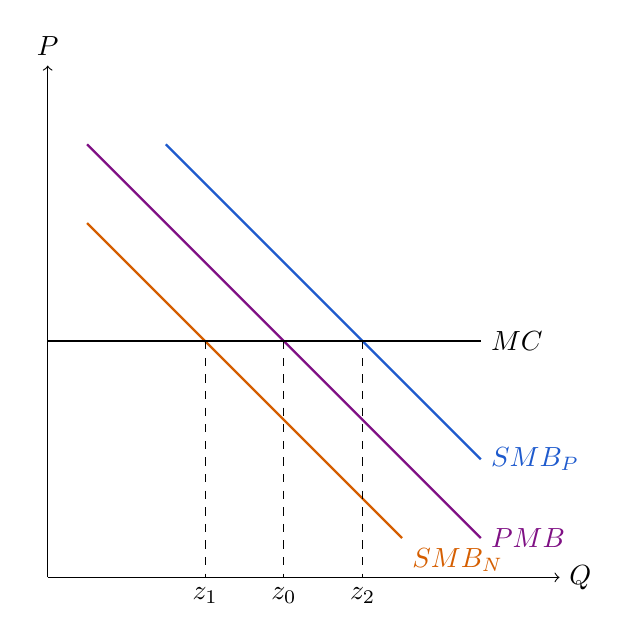
\begin{tikzpicture}[scale=1.0]
  %% 1. Axes
  \draw[->] (0,0) -- (6.5,0) node[right] {$Q$};
  \draw[->] (0,0) -- (0,6.5) node[above] {$P$};
  %% 2. Curves
  \draw[thick, color=NTHU1] (0.5,5.5) -- (5.5,0.5) node[right] {$PMB$};
  \draw[thick, color=blue] (1.5,5.5) -- (5.5,1.5) node[right] {$SMB_P$};
  \draw[thick, color=red] (0.5,4.5) -- (4.5,0.5) node[below right] {$SMB_N$};
  \draw[thick, color=black]  (0,3) -- (5.5,3) node[right] {$MC$};
  
\draw[dashed, color=black]  (4,3) -- (4,0) node[below] {$z_2$};
  \draw[dashed, color=black]  (2,3) -- (2,0) node[below] {$z_1$};
  \draw[dashed, color=black]  (3,3) -- (3,0) node[below] {$z_0$};
  %% 3. Points and labels
  
  %\filldraw[NTHU1] (3,2) circle (2pt) node[above] {$E$};
  %% 4. Shaded regions

\end{tikzpicture}
\end{column}
\begin{column}{0.55\textwidth}
Definition
\begin{itemize}\setlength\itemsep{3pt}
\item Externality: When cost or benefit on 3rd party is not reflected in market prices
\item Social marginal beneflt (SMB)\\ $\neq$ Private marginal benefit (PMB)
\end{itemize}\bigskip

Market vs socially optimal outcome
\begin{itemize}\setlength\itemsep{3pt}
\item Market: $PMB=MC$ $\to$ $z_0$
\item Positive externality: $SMB_P=MC$ $\to$  $z_1$
\begin{itemize}
  \item Markets underprovide the good
\end{itemize}
\item Negative externality: $SMB_N=MC$ $\to$  $z_2$
\begin{itemize}
  \item Markets overprovide the good
\end{itemize}
\end{itemize}
\end{column}
\end{columns}
\end{frame}


\begin{frame}
\frametitle{Mathematical analysis of externalities} 
Setup with two goods and two persons
\begin{itemize}\setlength\itemsep{3pt}
  \item Utility for both (good 2 ($z_i$) induces externality)
  \[
  \begin{aligned}
    U_1&= x_1 + u_1(z_1)+v_1(z_2)\\
    U_2&= x_2 + u_2(z_2)+v_2(z_1)
  \end{aligned}
  \]
  where if $v_i'>0\to$ positive externality and otherwise negative
  \item Individual and social budget constraints are as follows
  \[
  \begin{aligned}
    \text{Individual (IBC): }&x_i+pz_i \leq \omega_i \ \ \ (i\in\{1,2\}) \\
    \text{Social (SBC): }&x_1+x_2+pz_1+pz_2 \leq \omega_1+\omega_2
  \end{aligned}
  \]
\end{itemize}
\end{frame}

\begin{frame}
\frametitle{Mathematical analysis of externalities} 
Market outcomes
\begin{itemize}\setlength\itemsep{3pt}
  \item Each individual maximizes own utility subject to IBC
  \[
  \max_{x_i, z_i} x_i + u_i(z_i)+v_i(z_j) + \lambda[\omega_i - x_i-pz_i]
  \]\vspace{-10pt}
  \begin{itemize}\setlength\itemsep{3pt}
    \item FOC w.r.t [$x_i$]: $\lambda=1$
    \item FOC w.r.t [$z_i$]: $u_i'(z_i)-\lambda p=0 \Rightarrow u_i'(z_i)=p $
  \end{itemize}
  \item Each individual equates their own marginal benefits with marginal costs (price of $z$)
\end{itemize}
\end{frame}


\begin{frame}
\frametitle{Mathematical analysis of externalities} 
Optimal outcomes
\begin{itemize}\setlength\itemsep{3pt}
  \item From society's perspective, it maximizes (where SWF = sum of individual utility)
  \[
  \max_{x_1,x_2, z_1,z_2} x_1 +x_2 + u_1(z_1)+u_2(z_2)+v_1(z_2)+v_2(z_1) + \mu[\omega_1+\omega_2 - x_1-x_2-pz_1-pz_2]
  \]\vspace{-10pt}
  \begin{itemize}\setlength\itemsep{3pt}
    \item FOC w.r.t [$x_i$]: $\mu=1$ for any $i$
    \item FOC w.r.t [$z_1$]: $u_1'(z_1)+v_2'(z_2)-\mu p=0 \Rightarrow u_1'(z_1)+v_2'(z_1)=p $
    \item FOC w.r.t [$z_2$]: $u_2'(z_2)+v_1'(z_2)-\mu p=0 \Rightarrow u_2'(z_2)+v_1'(z_2)=p $
  \end{itemize}\smallskip
\item In positive externality $(v_i'(z_j)>0: SMB_P)$
 \begin{itemize}\setlength\itemsep{3pt}
    \item $SMB_P$ is above $PMB$: Too little consumption of $z$ compared to desired levels
  \end{itemize}   \smallskip 
\item In negative externality $(v_i'(z_j)<0: SMB_N)$
\begin{itemize}\setlength\itemsep{3pt}
    \item $SMB_N$ is below $PMB$: Too much consumption of $z$ compared to desired levels
  \end{itemize}    
\end{itemize}
\end{frame}


\begin{frame}
\frametitle{Possible solutions through internalization} 
Pigouvian taxation and internalization
\begin{itemize}\setlength\itemsep{3pt}
\item Note that socially optimal $z_1$ satisfies
\[
u_1'(z_1) + v_2'(z_1)=p
\]
\item Person 1 will internalize person 2's benefit from $z_1$ if price charged to person 1 $(q_1)$ is
\[
u_1'(z_1)=q_1 = p-v_2'(z_1) 
\]
\item Effectively charge tax (or provide subsidy) $t_1$ with
\[
t_1=q_1-p = -v_2'(z_1) 
\]
Note that if $v_2'(z_1)<0$ then $t_1>0$ (tax), otherwise $t_1<0$ (subsidy)
\item May need individualized prices $\to$ difficult to implement
\item Other solutions: Mandate quantity through quantity controls (govt needs perfect info)
\end{itemize}\medskip
\end{frame}


\begin{frame}
\frametitle{Back to public goods} 
Socially optimal provision of public goods
\begin{itemize}\setlength\itemsep{3pt}
\item Social utility comes from consumption of private goods $x$ and public good $z$
\[SWF:\ W(U_1(x_1,z), U_2(x_2,z)) = U_1(x_1,z)+U_2(x_2,z)
\]
\item To characterize feasible allocation, we use the production possibilities frontier
 \[
 PPF: \ F(x_1,x_2,z)=0, \Rightarrow x_1+x_2+z \leq E
 \]
 \item Social optimum is derived from following Lagrangian
\[
\mathcal{L}=U_1(x_1,z)+ U_2(x_2,z) +\lambda [E-x_1-x_2-z]
\]

\end{itemize}
\end{frame}

\begin{frame}
\frametitle{Back to public goods} 
Solutions
\begin{itemize}\setlength\itemsep{3pt}
    \item FOC w.r.t.\ $x_i$ ($i=1,2$): $[x_i]: \quad  U_{i,X_i} - \lambda  = 0 \implies U_{i,x_i}=\lambda $
    
    \item FOC w.r.t.\ $z$: $[z]: \quad  U_{1,z} + U_{2,z} -\lambda  = 0\implies (U_{1,z} + U_{2,z}) = \lambda$
    \item Since $\lambda = U_{1,x_1} = U_{2,x_2}$
    from $[x_i]$, substitute into $[z]$:
    \[
    U_{1,z} + U_{2,z} = U_{1,x_1} = U_{2,x_2}
    \]
    \item Dividing through by $\lambda$ and using
    $U_{1,x_1} = U_{2,x_2} = \lambda$:
    \[
    \frac{U_{1,z}}{U_{1,x_1}} +
    \frac{U_{2,z}}{U_{2,x_2}} = 1
    \]
    \item Since $MRS_i^{zx} = U_{i,z}/U_{i,x_i}$
    and $MRT = 1$ (linear PPF):
    \[
    \boxed{\sum_i MRS_i^{zx} = MRT^{zx}}
    \]
\end{itemize}
\end{frame}

\begin{frame}
\frametitle{Optimal provision of public goods} 
Samuelson Condition
    \[
    \sum_i MRS_i^{zx} = MRT^{zx}
    \]
\begin{itemize}\setlength\itemsep{3pt}
    \item Sum of individual value of $z$ in terms of $x$  = Cost of producing $z$ in terms $x$
    \item This contrasts with efficient private good consumption (call it $y$), where
    \[ MRS_i^{yx} = MRT^{yx} \]
    i.e. person $i$ need not consider person $j$
    \item Efficient allocation requires knowledge on true value of public goods to \textit{each} person
    \begin{itemize}\setlength\itemsep{3pt}
      \item This information is private: People can understate their value to free-ride
      \item This is a preference revelation problem (markets fail to induce people to be truthful) 
      \item This shows why private provision of public goods is difficult
    \end{itemize}
\end{itemize}
\end{frame}



\subsection{Effects of providing welfare}
\begin{frame}
\frametitle{Income maintenance program: Mathematical setup}
Individual's problem
\begin{itemize}\setlength\itemsep{3pt}
\item Maximize its utility w.r.t. budget constraint (labor earnings)
\[
\max_{X,L} u(X,L) \ \ \text{s.t. } \ X \leq w(T-L)
\]\vspace{-10pt}
\begin{itemize}
  \item $X$: Consumption 
  \item $L$: Leisure (time not spent working)
  \item $T$: Maximal time per day
  \item $w$: Wages (per hour)
  \item $T-L$: Labor (I will use $l$ interchangeably) 
\end{itemize}
\end{itemize} \medskip
Assumptions
\begin{itemize}
  \item $u_X>0, u_L>0, u_{XX}<0, u_{LL}<0$ ($X$ and $L$: Normal goods, diminishing marginal returns)
\end{itemize}
\end{frame}

\begin{frame}
\frametitle{Income maintenance program: Mathematical setup}
Income maintenance program
\begin{itemize}\setlength\itemsep{3pt}
\item Ensures individuals earn at least $G$ through this benefit formula
\[
B=\max[G-tE,0]
\]\vspace{-10pt}
\begin{itemize}
  \item $E$: Labor earnings ($w(T-L)=wl$)
  \item $t$: Tax rate on additional earnings
\end{itemize}
\end{itemize} \medskip
Revised individual problem
\begin{itemize}
  \item Budget constraint: $X\leq w(T-L)+B$, which can be written as
   \[
   X\leq \max[(1-t)w(T-L)+G,w(T-L)]
   \]
 \item Practical apprach: Solve Two lagrangian (for each BC) $\to$ Choose highest Utility  
\end{itemize}
\end{frame}




\begin{frame}
\begin{columns}
  \begin{column}{0.45\textwidth}
\frametitle{Income maintenance program and labor supply} 
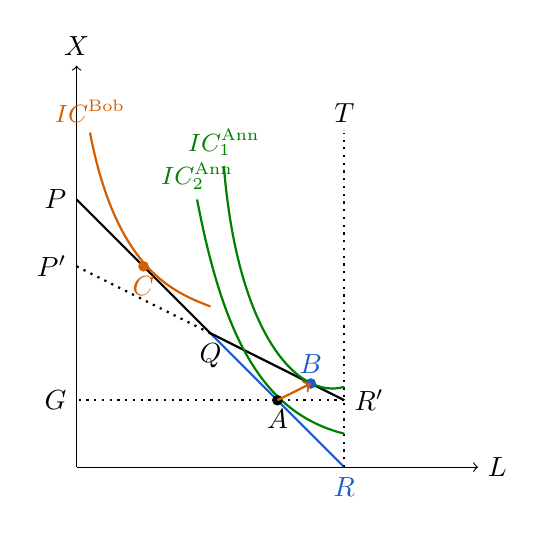
\begin{tikzpicture}[scale=0.85]
  \draw[->] (0,0) -- (6,0) node[right] {$L$};
  \draw[->] (0,0) -- (0,6) node[above] {$X$};
  %% Original budget line
  \draw[thick, blue] (4,0) node[below] {$R$}-- (2,2) ;
  \draw[thick, black] (2,2) -- (0,4) node[left] {$P$};
  %% Post-tax budget line
  \draw[thick, dotted, black] (0,3) node[left] {$P'$} -- (2,2) node[below] {$Q$};
  \draw[thick, black] (4,1) node[right] {$R'$} -- (2,2);
  \draw[thick, dotted,black] (4,1) -- (0,1) node[left] {$G$};
  \draw[thick, dotted,black] (4,0) -- (4,5) node[above] {$T$};
  %% Compensated (Hicksian) budget line — same slope as post-tax, tangent to original IC

  %% Indifference curves (hand-drawn approximations as bezier)
\draw[thick, green] (2.2,4.5) node[above] {\small $IC^{\text{Ann}}_1$} .. controls (2.4,2) and (3.3,1) .. (4,1.2) ;
  \draw[thick, green]  (1.8,4) node[above] {\small $IC^{\text{Ann}}_2$} .. controls (2.2,1.9) and (2.8,0.8) .. (4,0.5) ;

  \draw[thick, red]  (0.2,5) node[above] {\small $IC^{\text{Bob}}$} .. controls (0.6,2.9) and (1.5,2.6) .. (2,2.4) ;
  %% Three points
  \filldraw[black] (3,1) circle (2pt) node[below] {$A$};
  \filldraw[blue]  (3.5,1.25) circle (2pt) node[above ] {$B$};
  \draw[red, thick,->] (3,1) -- (3.5,1.25) ;
  \filldraw[red]  (1,3) circle (2pt) node[below] {$C$};
%  \filldraw[red]   (2.5,1) circle (2pt) node[below] {$B$};
  %% Braces
\end{tikzpicture}
\end{column}
\begin{column}{0.55\textwidth}
Visualizing income maintenance program
\begin{itemize}\setlength\itemsep{3pt}
\item Pre-program budget constraint: $PQR$
\item Post-program budget constraint: $PQR'$
\end{itemize}\medskip
Ann's choice
\begin{itemize}\setlength\itemsep{3pt}
\item Moves from $A$ to $B$
\item Consumption and leisure $\uparrow$, labor $\downarrow$
\item Effect of $t$ on labor: Substitution dominates
\begin{itemize}\setlength\itemsep{3pt}
\item Subsitution effect: labor $\downarrow$
 \item Income effect: labor $\uparrow$
\end{itemize}
\end{itemize}\medskip
Bob's choice
\begin{itemize}\setlength\itemsep{3pt}
\item Choice unaffected at $C$
\end{itemize}\medskip
\end{column}
\end{columns}
\end{frame}

\begin{frame}
\frametitle{Explaining labor disincentives}
How substitution effect works
\begin{itemize}\setlength\itemsep{3pt}
\item Recall the budget constraint
\[
   X\leq \max[(1-t)w(T-L)+G,w(T-L)]=\max[(1-t)wl+G,wl]
   \]\vspace{-20pt}
\item Without $t$: For additional unit of labor $l$, get $w$ 
\item With $t$: Additional unit of labor only returns $(1-t)w$
\item Larger $t$ $\to$ larger subsitution effect: Labor results in less budget (and comsuption)
\item Explains why many beneficients opt to not work
\end{itemize} \medskip
But these do not apply to everyone
\begin{itemize}\setlength\itemsep{3pt}
\item If $E>\frac{G}{t}$, budget constraint unaffected ($\because \max[G-tE,0]=0$, like Bob) 
\item $t$ \textit{may} raise labor through income effect
\begin{itemize}\setlength\itemsep{3pt}
\item Higher $t$ $\to$ Less income (poorer) $\to$ Less leisure (and subsequently more labor)
\item Overall effect of $t$ depends on relative strength of substitution and income effects
\end{itemize}
\end{itemize}
\end{frame}


\begin{frame}
\frametitle{Different types of income support program: Earned income tax credit} 
Design of EITC setup
\begin{itemize}\setlength\itemsep{3pt}
    \item Refundable tax credit for low-to-moderate income
    workers in the US
    \item EITC is conditional
    on earned income --- explicitly designed to reward work
    \item Benefit formula has three regions (based on labor income $y$)
    \begin{itemize}\setlength\itemsep{3pt}
        \item \textbf{Phase-in} $(y<G)$ : Credit rises with $y$ at rate $\tau_s$ until $G$ -- subsidize labor supply
        \item \textbf{Flat} $(G\leq y \leq G')$: Maximum credit $\tau_s \cdot G$ maintained over a $y$ between $G$ and $G'$
        \item \textbf{Phase-out} $(G'<y<G'')$: Credit withdrawn at rate $\tau_r$ for $y$ beyond $G'$, phased out at $G''$
    \end{itemize}
    \item Mathematic formula
        \begin{itemize}\setlength\itemsep{3pt}
        \item \textbf{Phase-in}: $w(T-L)+\tau_s w (T-L)$
        \item \textbf{Flat}: $w(T-L)+\tau_S G$
        \item \textbf{Phase-out}: $(1-\tau_r)w(T-L)+\tau_s G -\tau_r G'$
    \end{itemize}
    \item Encourage labour force participation while providing income support 
\end{itemize}
\end{frame}

\begin{frame}
\frametitle{EITC: Budget constraint and labor supply}
\begin{columns}
\begin{column}{0.45\textwidth}
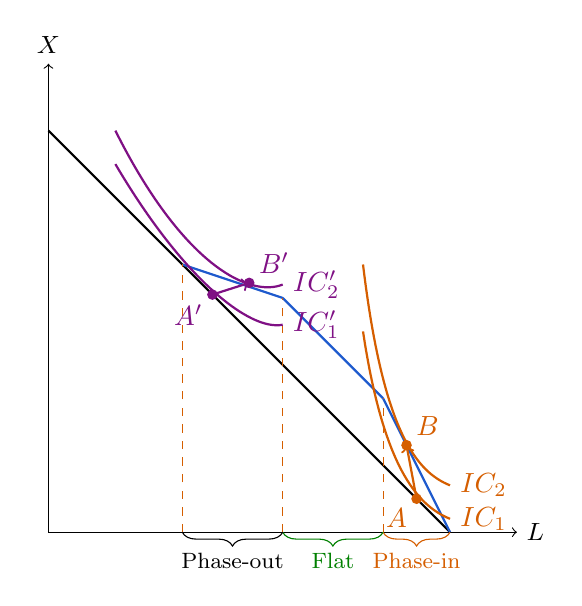
\begin{tikzpicture}[scale=0.85]
    \draw[->] (0,0) -- (7,0) node[right] {\small $L$};
    \draw[->] (0,0) -- (0,7) node[above] {\small $X$};

    %% Original budget line (black)
    \draw[thick, black] (0,6) -- (6,0) node[below] {};

    %% EITC budget line (kinked, lies above original)
    %% Phase-out (blue): from y-intercept, shallower slope
    \draw[thick, blue] (2,4) -- (3.5,3.5);
    %% Flat (black): horizontal segment at maximum credit
    \draw[thick, blue] (3.5,3.5) -- (5,2);
    %% Phase-in (red): steeper than original, meets original at B1
    \draw[thick, blue] (5,2) -- (6,0);

    %% Dotted vertical lines at kink points
    \draw[dashed, red] (2,0)  -- (2,4);
    \draw[dashed, red] (3.5,0) -- (3.5,3.5);
    \draw[dashed, red] (5,0)  -- (5,2);

    %% Indifference curve tangent at B3 (blue)
    %\draw[thick, blue]  (0.8,5.2) .. controls (1.5,3.5) and (2.5,2.5) .. (3.5,2.3);

    %% Indifference curve tangent at B2 (black)
   % \draw[thick, black] (1.5,4.8) .. controls (2.5,3.2) and (3.8,2.2) .. (5.0,2.0);

    %% Indifference curve tangent at B1 (red)
    \draw[thick, red]  (4.7, 4) .. controls (5,1.5) and (5.5,0.9) .. (6,0.7) node[right] {$IC_2$};
        \draw[thick, red]  (4.7, 3)  .. controls (5,1) and (5.5,0.4) .. (6,0.2) node[right] {$IC_1$};
  %% Three points
  \filldraw[red] (5.5,0.5) circle (2pt) node[below left] {$A$};
  \filldraw[red]  (5.35,1.3) circle (2pt) node[above right] {$B$};
  \draw[red, thick,->] (5.5,0.5) -- (5.35,1.3) ;

      \draw[thick, NTHU1]  (1, 6) .. controls (2,4) and (3,3.5) .. (3.5,3.7) node[right] {$IC'_2$};
        \draw[thick, NTHU1]  (1, 5.5)  .. controls (2,3.8) and (3,3) .. (3.5,3.1) node[right] {$IC' _1$};

        \filldraw[NTHU1] (2.45,3.55) circle (2pt) node[below left] {$A'$};
  \filldraw[NTHU1]  (3,3.725) circle (2pt) node[above right] {$B'$};
  \draw[NTHU1, thick,->] (2.45,3.55) -- (3,3.725) ;
    %% Tangency dots
  \draw[decorate, decoration={brace, amplitude=5pt}, red]
    (6,0) -- (5,0) node[midway, below=4pt] {\footnotesize Phase-in};
      \draw[decorate, decoration={brace, amplitude=5pt}, green]
    (5,0) -- (3.5,0) node[midway, below=4pt] {\footnotesize Flat};
      \draw[decorate, decoration={brace, amplitude=5pt}, black]
    (3.5,0) -- (2,0) node[midway, below=4pt] {\footnotesize Phase-out};
   % \filldraw[black] (3.5,3.0) circle (2pt);
   % \filldraw[red]   (6,0)     circle (2pt);

    %% Region labels on EITC line


\end{tikzpicture}
\end{column}
\begin{column}{0.55\textwidth}
Labor supply effects by region
\begin{itemize}\setlength\itemsep{3pt}
    \item \textbf{Phase-in}: effective wage
    $(1+\tau_s)w > w$
    \begin{itemize}
      \item Substitution effect: $l\Uparrow$
      \item Income effect: $l\Downarrow$ slightly
    \end{itemize}
    
    \item \textbf{Flat}: lump-sum transfer,
    effective wage $= w$
    \begin{itemize}
      \item  Income effect: $l\Downarrow$ slightly
      \item No substitution effect
    \end{itemize}
     
    \item \textbf{Phase-out}: effective wage
    $(1-\tau_r)w < w$
    \begin{itemize}
    \item Substitution and income effect: $l\Downarrow$
    \end{itemize}
    
\end{itemize}

\end{column}
\end{columns}
\end{frame}

\begin{frame}
\frametitle{Different types of income support program: Universal basic income} 

\begin{columns}
\begin{column}{0.45\textwidth}
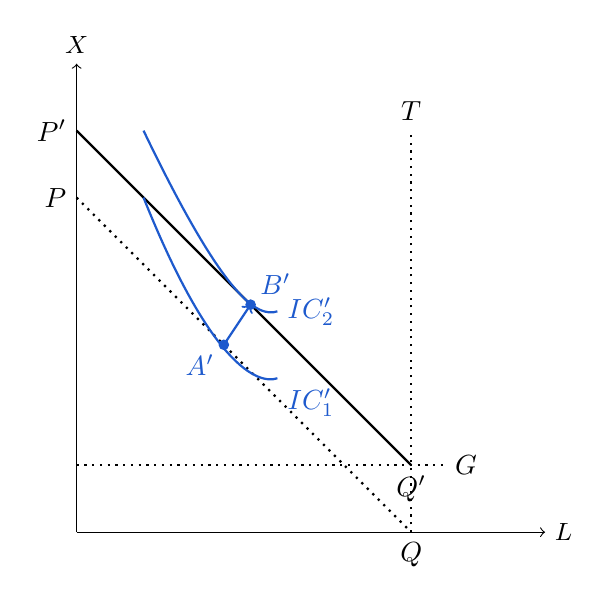
\begin{tikzpicture}[scale=0.85]
    \draw[->] (0,0)  -- (7,0) node[right] {\small $L$};
    \draw[->] (0,0) -- (0,7) node[above] {\small $X$};

    %% Original budget line (black)
    \draw[thick,dotted, black] (0,5) node[left] {$P$}-- (5,0) node[below] {$Q$};
    \draw[thick, black] (0,6) node [left] {$P'$}-- (5,1) node[below] {$Q'$};
    \draw[thick,dotted, black] (0,1) -- (5.5,1) node[right] {$G$};
    \draw[thick,dotted, black] (5,0) -- (5,6) node[above] {$T$};

    %% Indifference curve tangent at B3 (blue)
    %\draw[thick, blue]  (0.8,5.2) .. controls (1.5,3.5) and (2.5,2.5) .. (3.5,2.3);

    %% Indifference curve tangent at B2 (black)
   % \draw[thick, black] (1.5,4.8) .. controls (2.5,3.2) and (3.8,2.2) .. (5.0,2.0);

    %% Indifference curve tangent at B1 (red)
      \draw[thick, blue]  (1, 6) .. controls (2.2,3.5) and (2.7,3.2) .. (3,3.3) node[right] {$IC'_2$};
        \draw[thick, blue]  (1,5)  .. controls (2,2.5) and (2.7,2.2) .. (3,2.3) node[below right] {$IC' _1$};

        \filldraw[blue] (2.2,2.8) circle (2pt) node[below left] {$A'$};
  \filldraw[blue]  (2.6, 3.4) circle (2pt) node[above right] {$B'$};
  \draw[blue, thick,->] (2.2,2.8) -- (2.6,3.4) ;
    %% Tangency dots

   % \filldraw[black] (3.5,3.0) circle (2pt);
   % \filldraw[red]   (6,0)     circle (2pt);

    %% Region labels on EITC line


\end{tikzpicture}
\end{column}
\begin{column}{0.55\textwidth}
Changes in the constraints
\begin{itemize}\setlength\itemsep{3pt}
    \item Unconditional transfer $G$ to every
    individual
    \item Budget constraint simply shifts up by $G$
    \item  Effective wage unchanged $\Rightarrow$ \textit{no
    substitution effect}, only income effect
       \item Income effect predicts reduction in labor
    supply (leisure is a normal good)

\end{itemize} \medskip
Practical concerns
    \begin{itemize}\setlength\itemsep{3pt}
        \item Fiscal cost: universal coverage of $G$ requires high tax rates
        elsewhere
        \item Targeting: Transfers to non-poor
        households
    \end{itemize}
\end{column}
\end{columns}
\end{frame}

\begin{frame}
\frametitle{Different types of income support program: Negative income tax} 
Theoretical motivations behind all above income maintenance programs
\begin{itemize}\setlength\itemsep{3pt}
    \item Friedman (1962): government sets a guaranteed
    income $G$ and a tax rate $t$ on earnings
    \[
    T(E) = tE - G
    \]
    negative when $E < G/t$ (transfer), positive when
    $E > G/t$ (tax)
    \item The income maintenance program \textit{is} a NIT:
    $B = \max[G - tE, 0]$
    \item Special cases:
    \begin{itemize}\setlength\itemsep{3pt}
        \item EITC: adds a phase-in region where $t < 0$
        (subsidy on earnings) 
        \item UBI: sets $t = 0$ --- pure lump-sum $G$,
        no substitution effect, only income effect
    \end{itemize}
    \item All three share the same equity--efficiency trade-off 
    \begin{itemize}\setlength\itemsep{3pt}
        \item Higher $G$ improves redistribution but requires higher $t$ to finance
        \item Higher $t$ distorts labor supply through substitution effect
    \end{itemize}
\end{itemize}
\end{frame}

\begin{frame}
\frametitle{Different types of income support program: Unemployment insurance} 
Individuals pay a premium while working and receive benefits when unemployed
\begin{itemize}\setlength\itemsep{3pt}
\item Suppose that $\alpha$ percent of population is employed ($1-\alpha$ unemployed)
\begin{itemize}\setlength\itemsep{3pt}
  \item Assume that everyone has asset $A$ and have same utility function $u(\cdot)$
  \item If employed: Labor income $w$ with disutility $d$, pay premium $T$
  \[
  X_e \leq w-T+A
  \]
  \item If unemployed: No labor income, but receive benefit $B$
  \[
  X_u \leq A+B
  \]
\end{itemize}
\item Government: Finances the program with taxes from employed, thus the constraint
\[ 
\alpha T = (1-\alpha)B 
\]
\item Need to prevent employed population `mimicking' unemployed 
\[u(\text{employed})\geq u(\text{unemployed})\]
\end{itemize}\medskip
\end{frame}


\begin{frame}
\frametitle{Constraints in solving the social welfare problem for UI} 
Mathematical setup of the social welfare problem
\[
\max_{T,B} \alpha[u(w-T+A)-x] + [(1-\alpha)u(A+B)] \ \ \ \ \ \text{s.t.  } \begin{cases}
  \alpha T = (1-\alpha)B & \text{(BC)}\\
  u(w-T+A)-x \geq u(A+B) & \text{(IC)}
\end{cases}
\]
\begin{itemize}\setlength\itemsep{3pt}
\item We plug in the BC to write the optimazation as
\[
\begin{aligned}
\max_{B} \alpha\left[u\left(w-\frac{1-\alpha}{\alpha}B+A\right)-x\right] + [(1-\alpha)u(A+B)] \\
 \text{s.t.  } u\left(w-\frac{1-\alpha}{\alpha}B+A\right)-x \geq u(A+B) 
\end{aligned}
\]
\end{itemize}\medskip
\end{frame}


\begin{frame}
\frametitle{Outcome and implications of UI} 
If we ignore the IC (incentive compatibility) constraint
\begin{itemize}\setlength\itemsep{3pt}
\item First order condition w.r.t $B$
\[
\begin{aligned}
[B]:& -\alpha \frac{1-\alpha}{\alpha}u_b\left(w-\frac{1-\alpha}{\alpha}B+A \right) + (1-\alpha)u_b(A+B)=0\\
&\iff w-\frac{1-\alpha}{\alpha}B+A = A+B \\
&\iff \alpha w=B
\end{aligned}
\]
\item When this is added to individual budget constraints, consumption is equalized at
\[
X_u = A+ \alpha w, \ X_e = w-(1-\alpha)W+A = A+\alpha w \Rightarrow X_u=X_e
\]
\item Full insurance, but no incentives for anyone to work in this case
\end{itemize}
\end{frame}

\begin{frame}
\frametitle{Outcome and implications of UI} 
If we consider the IC (incentive compatibility) constraint
\[
\alpha\left[u\left(w-\frac{1-\alpha}{\alpha}B+A\right)-x\right] + [(1-\alpha)u(A+B)] +\lambda\left[u\left(w-\frac{1-\alpha}{\alpha}B+A\right)-x -u(A+B) \right]
\]
\begin{itemize}\setlength\itemsep{3pt}
\item First order condition w.r.t $\lambda$: IC becomes binding and $\lambda>0$ (Kuhn-Tucker condition)
\[
\begin{aligned}
[\lambda]:  u(w-T+A)-x = u(A+B)
\end{aligned}
\]
\item First order condition w.r.t $B$: 
\[
\begin{small}
\begin{aligned}
[B]:& -u_B\left(w-\frac{1-\alpha}{\alpha}B+A\right)+u_B(A+B)=\lambda\left[\frac{u_B(w-\frac{1-\alpha}{\alpha}B+A)}{\alpha}+\frac{u_B(A+B)}{1-\alpha}\right]>0\\
&\Rightarrow A+B < A-\frac{1-\alpha}{\alpha}B+w \ \ (\text{or } X_u<X_e)\Rightarrow B <\alpha w
\end{aligned}
\end{small}
\]
\item Incentive compatible, but partial insurance $\to$ possible mimicking leads to second-best 
\end{itemize}
\end{frame}


\begin{frame}
\frametitle{Takeaways from public goods provision} 
Governments can correct for market failures
\begin{itemize}\setlength\itemsep{3pt}
\item Can achieve socially optimal allocation of public goods
\item Also provide redistribution (through different mechanisms)
\end{itemize}\medskip
However, even some socially optimal outcome are unachievable by government
\begin{itemize}\setlength\itemsep{3pt}
\item Governments also suffer from asymmetrical information problems
\item For solutions that require private information, government may not do better
\begin{itemize}
\item Any deviation from perfect competition $\to$ first-best solution are unachievable in any case
\end{itemize}
\item We also assume that government can implement any plans 
\begin{itemize}\setlength\itemsep{3pt}
\item Governments do create inefficient spending
\item The bureaucratic personnel and adminstrative backdrop may not be capable
\end{itemize}
\end{itemize}
\end{frame}



\section{Management of public services in reality}
\subsection{Liebman, Mahoney (2017): Do Expiring Budgets Lead to Wasteful Year-End Spending? Evidence from Federal Procurement }
\begin{transitionframe}
\begin{center}
  \begin{huge}
    \textcolor{NTHU1}{%
Liebman, Mahoney (2017): \\ Do Expiring Budgets Lead to Wasteful Year-End Spending? Evidence from Federal Procurement 
    }
  \end{huge}
\end{center}
\end{transitionframe}


\begin{frame}
\frametitle{Q: Do organizations spend wastefully at end of the year?} 
Decision structure at organizations
\begin{itemize}\setlength\itemsep{3pt}
\item Budgets expire at end of fiscal year (remainder are returned)
\item Organizations rush to spend that money, even at low-value projects
\begin{itemize}\setlength\itemsep{3pt}
  \item Low opportunity costs: These funds are unusable next year
\end{itemize}
\item Liquidity-constrained through out the year: Hold back expenditure early, spend late
\end{itemize}\medskip
This paper examines the cause and consequences of year-end spending
\begin{itemize}\setlength\itemsep{3pt}
\item Uses US federal government procurement data
\item Documents increasing late-year spending (vs other parts of the year)
\item Drop-off in quality of projects spent on at late-year
\item Policy suggestion: Allow for rollover to next year (some departments do)
\end{itemize}
\end{frame}

\begin{frame}
\frametitle{Simple model} 
Budgeting model for the government agency
\begin{itemize}\setlength\itemsep{3pt}
\item An agency makes the spending ($x_m$) decision  for each half-year ($m\in\{1,2\}$)
\item The spending generates $\alpha_m v(x_m)$ value ($\alpha_m$: stochastic, $v$ is concave)
\item The funds are allocated to the agency by the congress
\item Agency solves 
\[
\max_{x_1,x_2} \alpha_1 v(x_1)+E_{\alpha_2}[\alpha_2 v(x_2)] \ \ \   \text{s.t. }\ \ \ \ x_1+x_2\leq B
\]
\item Congress solves at beginning of each year
\[
\max_B E_{\alpha_1, \alpha_2}[\alpha_1 v(x_1)+\alpha_2 v(x_2)-\lambda(x_1^*+x_2^*)]
\]
\item Due to concavity of $v$ and uncertainty about $m=2$ at planning, $x_2^*>x_1^*$
\item Due to high $x_2$ and cocavity of $v$, quality of spending ($\alpha_mv(x_m)/x_m$) is lower in $m=2$
\end{itemize}\medskip
\end{frame}



\begin{frame}
\frametitle{Data sources and empirical strategy} 
Data from federal procurement data (2004-2009)
\begin{itemize}\setlength\itemsep{3pt}
\item USAspending.gov is the primary source (for all contracts)
\item Total value of contract, and breakdown of costs are available
\item Available across multiple government branches (for quality analysis, rely on IT projects)
\end{itemize}\medskip
Regression analysis
\begin{itemize}\setlength\itemsep{3pt}
\item Quality analysis: Ordered logit regression
\begin{itemize}\setlength\itemsep{3pt}
  \item Odds ratio as outcome: Odds ratio 1/2 = chances of higher categorical value is 50\% lower 
  \item Conversely, it means odds of lower category are 2 times as great
\end{itemize}
\item Effect of rollovers: Department of justice (with rollover) vs others around 1992
 \begin{itemize}\setlength\itemsep{3pt}
  \item DOJ authorized to rollover 4\% of annual revenue in 1992 for IT projects
  \item Compare 1994-2006 period spending
\end{itemize}
\end{itemize}\medskip
\end{frame}



\begin{frame}
\frametitle{Spending bunched at the end of fiscal year} 
\begin{figure}
  \includegraphics[keepaspectratio, width=0.8\textwidth]{lm(2017)_f1.jpg}
\end{figure}
\end{frame}

\begin{frame}
\frametitle{Chances of low quality investment: 2.3-5.6 times higher at last  week} 
\begin{figure}
  \includegraphics[keepaspectratio, width=0.67\textwidth]{lm(2017)_t1.png}
\end{figure}
\begin{itemize}
  \item Inverse of 0.18 and 0.43 are 5.6 and 2.3, respectively
\end{itemize}
\end{frame}

\begin{frame}
\frametitle{Rollover reduces year-end spending by 9.5 percentage points} 
\begin{figure}
  \includegraphics[keepaspectratio, width=0.8\textwidth]{lm(2017)_t2.png}
\end{figure}
\end{frame}


\subsection{Rasul, Rogger (2018): Management of Bureaucrats and Public Service Delivery: Evidence from Nigerian Civil Service}
\begin{transitionframe}
\begin{center}
  \begin{huge}
    \textcolor{NTHU1}{%
Rasul, Rogger (2018): \\ Management of Bureaucrats and Public Service Delivery: Evidence from Nigerian Civil Service
    }
  \end{huge}
\end{center}
\end{transitionframe}


\begin{frame}
\frametitle{Q: Do management practices matter for public organizations?} 
Government effectiveness matters, but what contributes to it?
\begin{itemize}\setlength\itemsep{3pt}
\item Economic analysis in public sector focused on selection and incentives
\item Not much on managerial practices applied to middle-tier of bureaucrats
\end{itemize}\medskip
This study estimates correlation between public service and management practices 
\begin{itemize}\setlength\itemsep{3pt}
\item Background: Nigeria (Largest population in Africa, has inefficient practices)
\item Data collected through survey on management practices and outputs of agencies
\item Better autonomy increases completion rates (incentive/monitoring does the opposite)
    \begin{itemize}\setlength\itemsep{3pt}
  \item Incentives are misaligned, 
  \item Bureaucrats spend more time gathering performance indicators vs actually working
\end{itemize}
\end{itemize}

\end{frame}

\begin{frame}
\frametitle{Data sources and empirical strategy} 
Primary datasets
\begin{itemize}\setlength\itemsep{3pt}
\item Details on 4700 public sector projects (since 2006) handcoded  (8\% of social spending)
\item Above data are from civil society members and independent engineers
\item Management practice from surveys on Nigerian public sector workers
\begin{itemize}
  \item Focus on autonomy (have say in input, flexibility) vs incentives and monitoring
\end{itemize}
\end{itemize}\medskip
Research design exploits variation in practices across organizations doing similar projects
\[
y_{ijn}=\gamma_1\text{Autonomy}_n+\gamma_2\text{Inc/Mon}_n+\gamma_3\text{other}_n+\beta X_{ijn} + \lambda_j+e_{ijn}
\]\vspace{-20pt}
\begin{itemize}\setlength\itemsep{3pt}
  \item $i$:project, $j$: project type, $n$: organization
  \item e.g. Small dams constructed by three different organizations
  \item Outcome: Project completion rates (note: 30+\% of projects not even started in NGA)
  \item Does not fully control for endogenous selection of projects
   \begin{itemize}
  \item Still have non-random differences across autonomy vs incentive/monitoring practices
\end{itemize}
\end{itemize}
\end{frame}


\begin{frame}
\frametitle{Project completion correlated with management practices} 
\begin{figure}
  \includegraphics[keepaspectratio, width=1\textwidth]{rr(2018)_t1.png}
\end{figure}
\end{frame}

\begin{frame}
\frametitle{Why might incentive-based practices be ineffective?} 
Heterogeneity analysis (Table 5 in the paper)
\begin{itemize}\setlength\itemsep{3pt}
\item Negative effects exacerbated for more complex projects
\begin{itemize}\setlength\itemsep{3pt}
  \item These require more varied effort types to be exerted
  \item Difficult to target and design optimal incentives schemes (all else equal)
\end{itemize}
\item Older bureaucrats respond to incentivs with influence activities (vs. actual work)
\item Also worse if we have subjective (not objective) performance evaluation
\item Suggestive evidence of roles played by corruption
\end{itemize}\medskip

\end{frame}


\begin{frame}
\frametitle{Incentives geared towards engaging with politicians vs actual work} 
\begin{figure}
  \includegraphics[keepaspectratio, width=1\textwidth]{rr(2018)_t2.png}
\end{figure}
\end{frame}


\begin{frame}
\frametitle{Next class} 
Moving onto the develping country contexts
\begin{itemize}\setlength\itemsep{3pt}
\item Opportunity to observe Classical theoretical format more critically
\item Identify what can still carry over
\item More importantly, examine what \textit{does not} carry over to developing countries
\end{itemize}\medskip
 Key topics (for the remainder of this course)
\begin{itemize}\setlength\itemsep{3pt}
\item Fiscal capacity in developing countries 
\item Anti-poverty programs in developing countries
\item Organization of public institutions
\end{itemize}\medskip
\end{frame}

%%%%%%%%%%%
\end{document}
